\documentclass[polish,aspectratio=169]{beamer}

% wide screen
% \documentclass[aspectratio=169]{beamer}


%%% YOUR PACKAGES HERE %%%
\usepackage{comment}
\usepackage{hyperref}
\usepackage[backend=biber, style=numeric, bibstyle=ieee,
            sorting=none, isbn=false, urldate=ymd,
            doi=false, url=true]{biblatex}
\addbibresource{bibliography/bibliography.bib}
\renewbibmacro{in:}{}
\usepackage{subfigure}
\usepackage{graphicx}
\usepackage{geometry}
\usepackage{float}
\usepackage{listings}
\usepackage{xcolor}

\newcommand{\refrys}[1]{Rys.~\ref{#1}}
\newcommand{\reflist}[1]{List.~\ref{#1}}
\newcommand{\refEq}[1]{Równ.~\ref{#1}}
% \usepackage{tikz} 
% \usetikzlibrary{graphs,graphs.standard,automata}


% polish language
% \usepackage[polish]{babel}
% \usepackage{polski}



%%% IMPORT PG PRESENTATION STYLE %%%
% THIS IS GDANSK UNIVERSITY OF TECHNLOGOGY (PG) PRESENTATION TEMPLATE
% Creator: Jan Cychnerski <jan.cychnerski@eti.pg.edu.pl>
% Copyleft 2019


% PG THEME OPTIONS

\usetheme{Boadilla}
\usecolortheme{default}
\usefonttheme{professionalfonts}

% colors

\definecolor{PGBlue}{RGB}{0,56,101}
\definecolor{PGRed}{RGB}{193,10,39}
\definecolor{PGSilver}{RGB}{200,200,200}
\definecolor{PGBlack}{RGB}{0,0,0}

% PGBlue
\setbeamercolor{frametitle}{fg=PGBlue}
\setbeamercolor{normal text}{fg=PGBlue}
\setbeamercolor{structure}{fg=PGBlue}
\setbeamercolor{item}{fg=PGBlue}

% PGRed
\setbeamercolor{alerted text}{fg=PGRed}
\setbeamercolor{item projected}{fg=PGRed}

% white
\setbeamercolor{title}{fg=white}
\setbeamercolor{titlelike}{fg=white}
\setbeamercolor{subtitle}{fg=white}

% enumerate and itemize styles

\setbeamertemplate{itemize item}{\bfseries\color{PGRed}\raise1pt\hbox{\donotcoloroutermaths$\bullet$}}
\setbeamertemplate{itemize subitem}{\color{PGRed}\raise0.5pt\hbox{--}}
\setbeamertemplate{itemize subsubitem}{\color{PGRed}\tiny\raise1.5pt\hbox{\donotcoloroutermaths$\bullet$}}

\setbeamertemplate{enumerate item}{\bfseries\color{PGRed}\insertenumlabel.}
\setbeamertemplate{enumerate subitem}{\color{PGRed}\insertsubenumlabel.}
\setbeamertemplate{enumerate subsubitem}{\color{PGRed}\insertsubsubenumlabel.}
\setbeamertemplate{enumerate mini template}{\insertenumlabel}


% disable navigation

\beamertemplatenavigationsymbolsempty

% additional commands

\newcommand*{\vcenteredhbox}[1]{\begingroup
\setbox0=\hbox{#1}\parbox{\wd0}{\box0}\endgroup}

\graphicspath{{pgbeamer/}}


\usepackage{iflang}
\IfLanguageName{polish}{
\newcommand{\pglogobig}{pg-logo-big-pl}
\newcommand{\pglogosmall}{pg-logo-small-pl}
}{
\newcommand{\pglogobig}{pg-logo-big-en}
\newcommand{\pglogosmall}{pg-logo-small-en}
}


% FRAME TITLE LOGO
\addtobeamertemplate{frametitle}{\vcenteredhbox{\includegraphics[height=8mm]{\pglogosmall}}\bfseries}{}


\newcommand{\pgtitleframe}{{
% PG TITLE PAGE

\setbeamercolor{background canvas}{bg=PGBlue}
\setbeamercolor{title}{fg=white}
\setbeamercolor*{date}{fg=white}
\setbeamercolor*{author}{fg=white}

\setbeamertemplate{footline}{}

\begin{frame}[noframenumbering]
\centering
\vspace{1cm}
\includegraphics[height=3cm]{\pglogobig}
\vspace{5mm}
\maketitle
\end{frame}
}}

\newcommand{\pglastframe}{{
% PG LAST PAGE

\setbeamercolor{background canvas}{bg=PGBlue}
\setbeamercolor{title}{fg=white}
\setbeamercolor*{date}{fg=white}
\setbeamercolor*{author}{fg=white}

\setbeamertemplate{footline}{}

\begin{frame}[noframenumbering]
\centering
\vspace{1cm}
\includegraphics[height=5cm]{\pglogobig}
\end{frame}
}}



%%% YOUR OPTIONS HERE %%%

\title[Selected unusual provisions in the EULA]{Selected unusual provisions in the EULA}
\subtitle{}
\author{Marek Borzyszkowski \and Paulina Brzęcka}
\date{\today}

\setbeamercovered{invisible}
\begin{document}

\pgtitleframe


\begin{frame}{What is EULA (End User License Agreement)?}
  \begin{itemize}
    \item A legal contract between the software developer and the end user.
    \item Grants the user the right to use the software under specific terms.
    \item Often displayed during installation or first launch.
    \item Typically non-negotiable ("take-it-or-leave-it")\cite{DEFINITION}.
  \end{itemize}
\end{frame}

\begin{frame}{EULA vs. Terms of Service (ToS)}
  \begin{table}[h!]
    \centering
    \begin{tabular}{|l|p{5cm}|p{7cm}|}
    \hline
    \textbf{Aspect} & \textbf{EULA} & \textbf{Terms of Service (ToS) / Terms \& Conditions (T\&C)} \\
    \hline
    \textbf{Scope} & Focused on \textbf{software usage rights} & Broader: website, service, and platform rules \\
    \hline
    \textbf{Target} & Individual \textbf{software users} & Website/app users, consumers, community members \\
    \hline
    \textbf{Binding} & Usually shown during installation & Often on websites (agreed via use) \\
    \hline
    \textbf{Example} & Microsoft Windows EULA & Facebook Terms of Service \\
    \hline
    \end{tabular}
    \caption{Comparison between EULA and Terms of Service\cite{TOS}}
  \end{table}
\end{frame}

\begin{frame}{Why are EULAs Rarely Read?}
    \begin{itemize}
      \item Too long and full of legal jargon.
      \item Presented during moments when users are eager to proceed (e.g., install).
      \item Click-through agreements make it easy to skip reading.
      \item Psychological: “Everyone else accepts, so I do too.”\cite{RARE}
    \end{itemize}
    \begin{alertblock}{Interesting fact}
      A study by Carnegie Mellon University estimated that reading all the privacy policies encountered annually would take the average user 76 workdays\cite{FACT}.
    \end{alertblock}
\end{frame}

\begin{frame}{Why are EULAs Rarely Read?}
\begin{columns}[c]
    \column{.5\textwidth}
    \centering
    \begin{figure}
        \centering
        
\includegraphics[width=0.65\textwidth]{images/dog.png}
        \label{fig:dog}
    \end{figure}  
    \column{.5\textwidth}
    \centering
    \begin{figure}
        \centering
        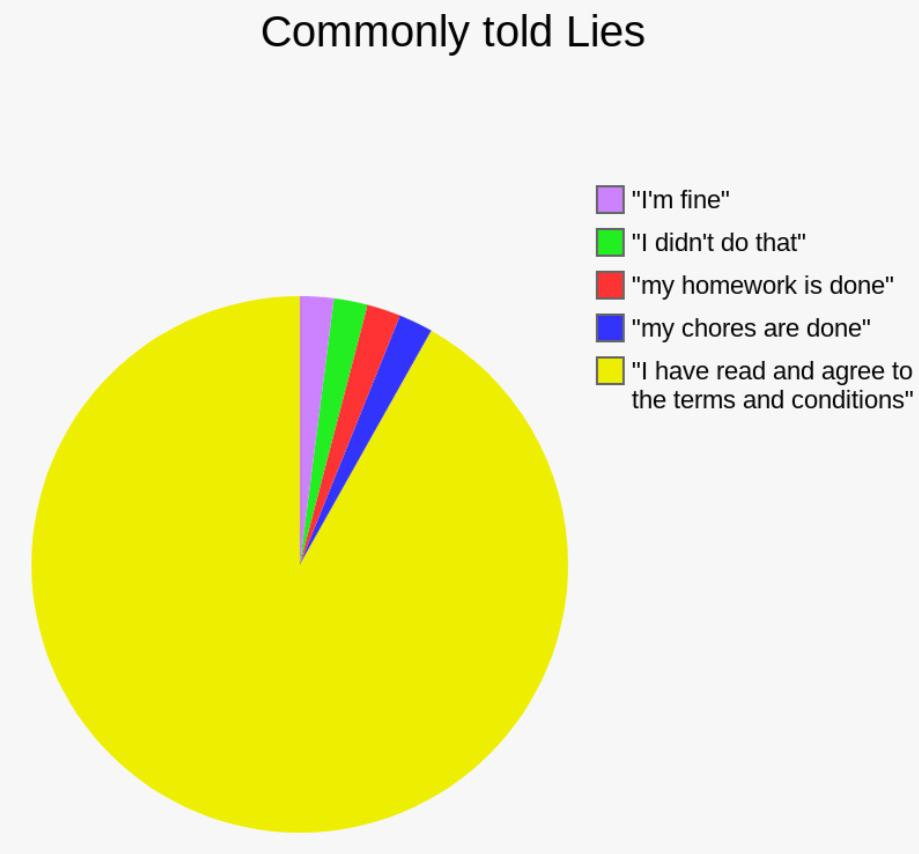
\includegraphics[width=\textwidth]{images/lies.jpg}
        \label{fig:lies}
    \end{figure}    
\end{columns}
\end{frame}

% \begin{frame}{Amazon}
    \begin{columns}[c]
        \column{.4\textwidth}
        \begin{figure}
            \centering
            
\includegraphics[height=0.40\textheight]{images/Lumberyard_Logo.png}
            \caption{AWS Lumberyard logo \cite{AWS_Lumberyard_logo}}
            \label{fig:AWS_Lumberyard}
        \end{figure}
        \column{.6\textwidth}
        \begin{figure}
            \centering
            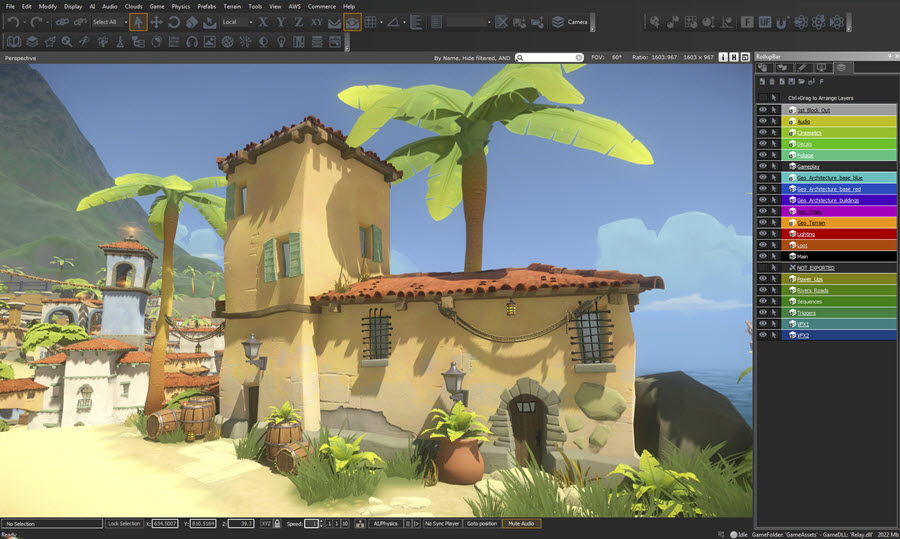
\includegraphics[height=0.60\textheight]{images/lumberyard_editor_relay_1.jpg}
            \caption{AWS Lumberyard \cite{AWS_Lumberyard_view}}
            \label{fig:social-media}
        \end{figure}
    \end{columns}
\end{frame}
    

\begin{frame}{Amazon}
    \begin{quote}
    "The terms state that Lumberyard is not to be used with \textbf{drones, medical equipment, nuclear facilities, manned spacecraft or live military combat} in normal times, but have a special exception.   
    \end{quote}  
    \pause
    \begin{quote}
        "Clause 57.10 of the AWS terms of service states: “This restriction will not apply in the event of the occurrence (certified by the United States Centers for Disease Control or successor body) 
        of a \textbf{widespread viral infection transmitted via bites or contact with bodily fluids that causes human corpses to reanimate and seek to consume living human flesh, blood, brain or nerve tissue} and is 
        likely to result in the fall of organised civilisation.”"    
    \end{quote}
    \mbox{}\hfill\textit{--- Amazon AWS EULA, 2016}      \cite{GUARDIAN_AWS_ZOMBIE}
\end{frame}

\begin{frame}{Gamestation}
    \begin{columns}[c]
        \column{.55\textwidth}
        \begin{block}{UK video‑game retailer \emph{Gamestation}, \textit{1~April~2010} (April Fools' Day):}
            \begin{itemize}
               \item Added an \emph{``Immortal Soul Clause''} to the online Terms\&Conditions, claiming legal ownership of each buyer's soul.
            \item Experiment highlighting how rarely people read EULAs/T\&Cs.
            \item \textbf{Results}
                \begin{itemize}
                \item \textbf{7,500} transactions that day
                \item \alert{88\%} accepted without noticing
                \item \alert{12\%} spotted the clause and received a \pounds5 gift voucher
                \end{itemize}
            \item Gamestation emailed all buyers, \emph{releasing} their souls and urging them to read future contracts.
    
            \end{itemize}
        \end{block}
        \column{.45\textwidth}
        \begin{figure}
            \centering
            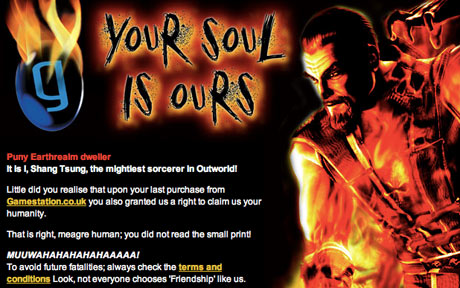
\includegraphics[height=0.50\textheight]{images/gamestation.jpg}
            \caption{Gamestation email \cite{Soul_EULA}}
            \label{fig:soul}
        \end{figure}
    \end{columns}
\end{frame}

    
    
\begin{frame}{PC Pitstop's \$1,000 EULA Experiment}
\begin{itemize}
    \item In 2005, PC Pitstop added a hidden clause in its EULA:
    \begin{quote}
        “If you’re reading this and contact us, you may receive money.”
    \end{quote}
    \item Over \textbf{3,000 downloads} later, only \textbf{1 person} noticed—and won \textbf{\$1,000}.
    \item Purpose: Show that users rarely read EULAs.
\end{itemize}

\vspace{0.3cm}
\textit{Proof: Even with an incentive, almost no one reads license agreements.\cite{MONEY}}
\end{frame}

\begin{frame}{Tumblr: Telling It Like It Is}

Tumblr humanizes legal content — a reminder that \textit{Terms of Service don’t have to be soulless}.
    \begin{columns}[c]
    \column{.8\textwidth}
    \begin{figure}
        \centering
        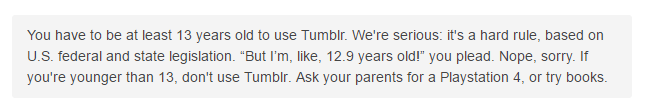
\includegraphics[width=\textwidth]{images/kids.png}
        \label{fig:kids}
    \end{figure}  
    \begin{figure}
        \centering
        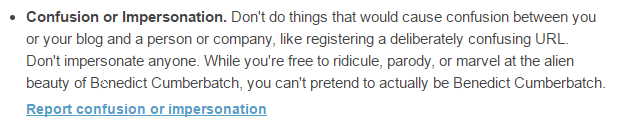
\includegraphics[width=\textwidth]{images/impersonate.png}
        \label{fig:impersonate}
    \end{figure}   
    \column{.2\textwidth}
    \centering
    \begin{figure}
        \centering
        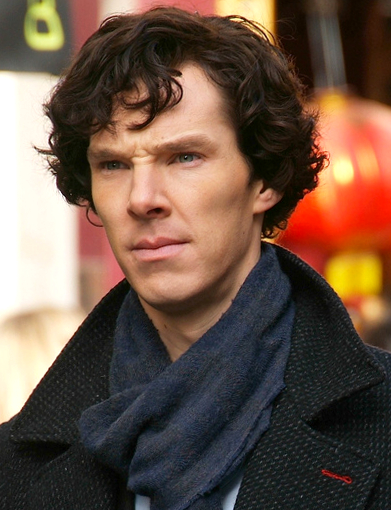
\includegraphics[width=\textwidth]{images/benedict.jpg}
        \label{fig:benedict}
    \end{figure}    
\end{columns}
\end{frame}

\begin{frame}{Tumblr: Telling It Like It Is}

Tumblr humanizes legal content — a reminder that \textit{Terms of Service don’t have to be soulless}\cite{TUMBLR}.
     \begin{figure}
        \centering
        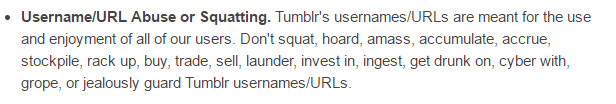
\includegraphics[width=\textwidth]{images/username.png}
        \label{fig:username}
    \end{figure}     
     \begin{figure}
        \centering
        
\includegraphics[width=\textwidth]{images/affirmation.png}
        \label{fig:affirmation}
    \end{figure}     
\end{frame}
% \begin{frame}{Rezultaty graczy na giełdzie}
    \begin{columns}[t]
        \column{.5\textwidth}
            wyniki
        \column{.5\textwidth}
        \centering
        \begin{figure}
            \centering
            
\includegraphics[width=1\textwidth]{images/aws_logo.png}
            \caption{obrazek}
            \label{fig:pic}
        \end{figure}    
    \end{columns}
\end{frame}

\begin{frame}{Community Service for free WiFi}
\begin{columns}[c]
    \column{.5\textwidth}
    \begin{itemize}
    \item Purple added a fake clause to its WiFi Terms: \textbf{1,000 hours of community service}.
    \item Tasks included:
    \begin{itemize}
        \item Cleaning toilets at festivals
        \item Hugging stray animals
        \item Scraping gum off streets
    \end{itemize}
    \item Over \textbf{22,000 users accepted}; only \textbf{1 person} noticed.
\end{itemize}

\vspace{0.2cm}
\textit{Goal: Show how blindly users click “I Agree.”} 
    \column{.5\textwidth}
    \centering
    \begin{figure}
        \centering
        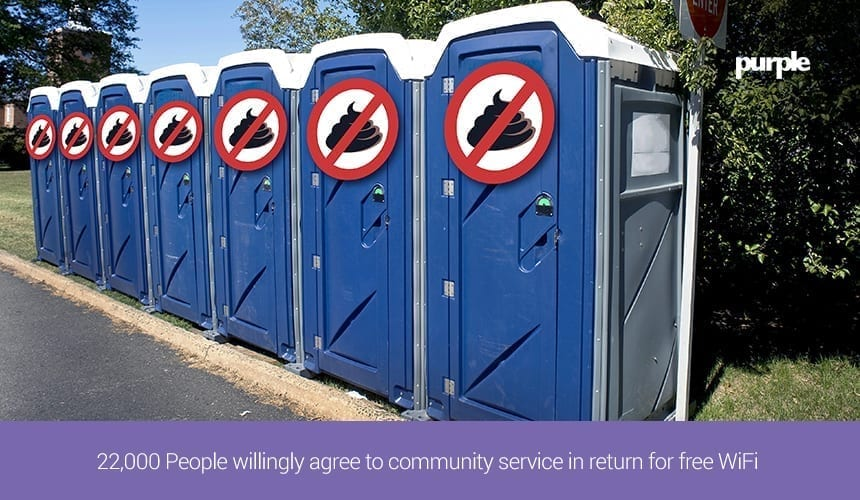
\includegraphics[width=\textwidth]{images/toilet.png}
        \label{fig:toilet}
    \end{figure}    
\end{columns}
\end{frame}

\begin{frame}{Lesson}
\begin{columns}[c]
    \column{.65\textwidth}
    \begin{itemize}
    \item Experiment raised awareness of careless digital consent.
    \item Inspired changes:
    \begin{itemize}
        \item Privacy policy shortened from 1,600 to 260 words.
        \item Clearer data usage explanations.
        \item Launch of a user-controlled Profile Portal \cite{TOILET}.
    \end{itemize}
\end{itemize}
    \column{.35\textwidth}
    \centering
    \begin{figure}
        \centering
        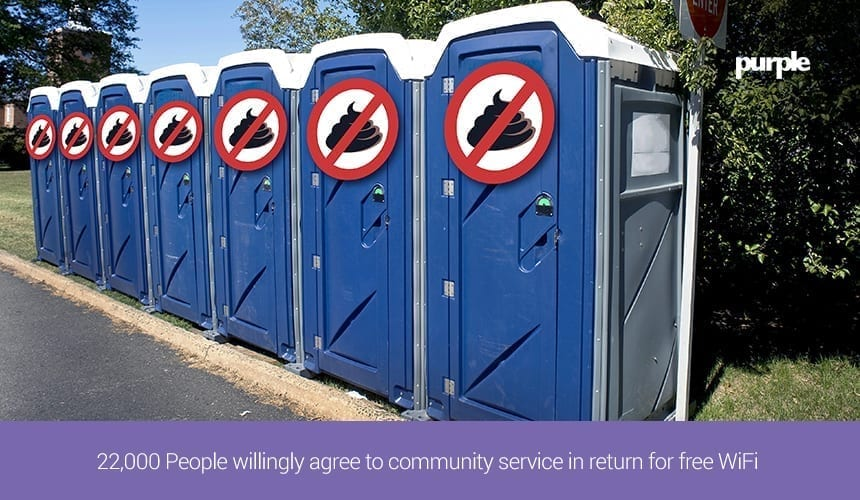
\includegraphics[width=\textwidth]{images/toilet.png}
        \label{fig:toilet}
    \end{figure}    
\end{columns}
\end{frame}

\begin{frame}{The Herod Clause}
\begin{columns}[c]
    \column{.5\textwidth}
  \begin{itemize}
    \item In June 2014, researchers set up public Wi-Fi hotspots in London.
    \item Users had to accept T\&Cs to get access.
    \item One clause (the “Herod Clause”) stated:
    \begin{quote}
        “You agree to assign your first born child to us for the duration of eternity.”
    \end{quote}
    \item \textbf{6 people accepted the terms} without noticing.
    \item Clause was later removed — the children were “returned.”
\end{itemize}

    \column{.5\textwidth}
    \centering
    \begin{figure}
        \centering
        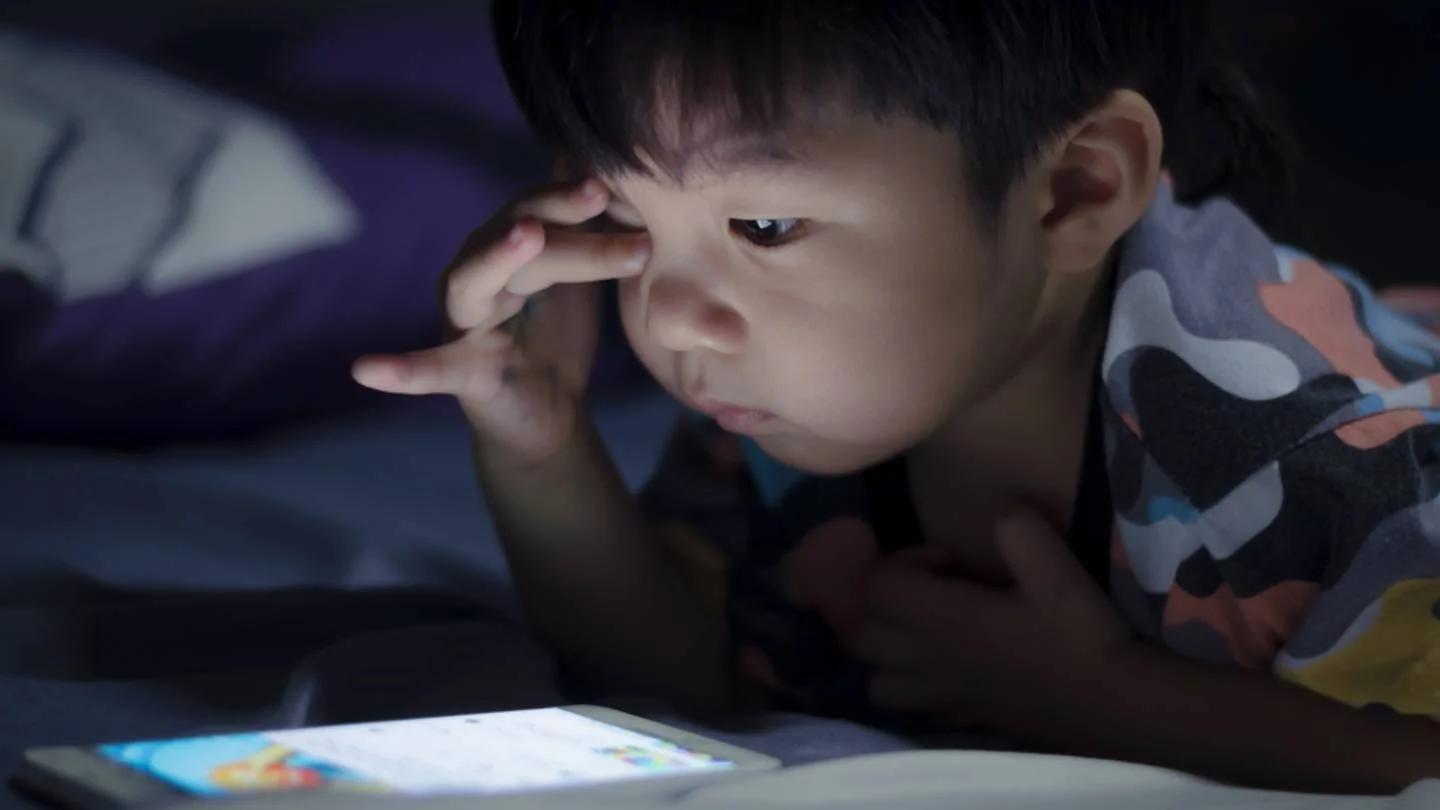
\includegraphics[width=\textwidth]{images/child.png}
        \label{fig:child}
    \end{figure}    
\end{columns}
\end{frame}

\begin{frame}{Why This Matters}
\begin{columns}[c]
    \column{.5\textwidth}
  \begin{itemize}
    \item Experiment run by the Cyber Security Research Institute and F-Secure.
    \item Goal: Raise awareness of careless public Wi-Fi use.
    \item Highlights two key issues:
    \begin{itemize}
        \item \textbf{Blind acceptance} of legal agreements.
        \item \textbf{Lack of awareness} about security risks in public networks\cite{CHILD}.
    \end{itemize}
\end{itemize}

    \column{.5\textwidth}
    \centering
    \begin{figure}
        \centering
        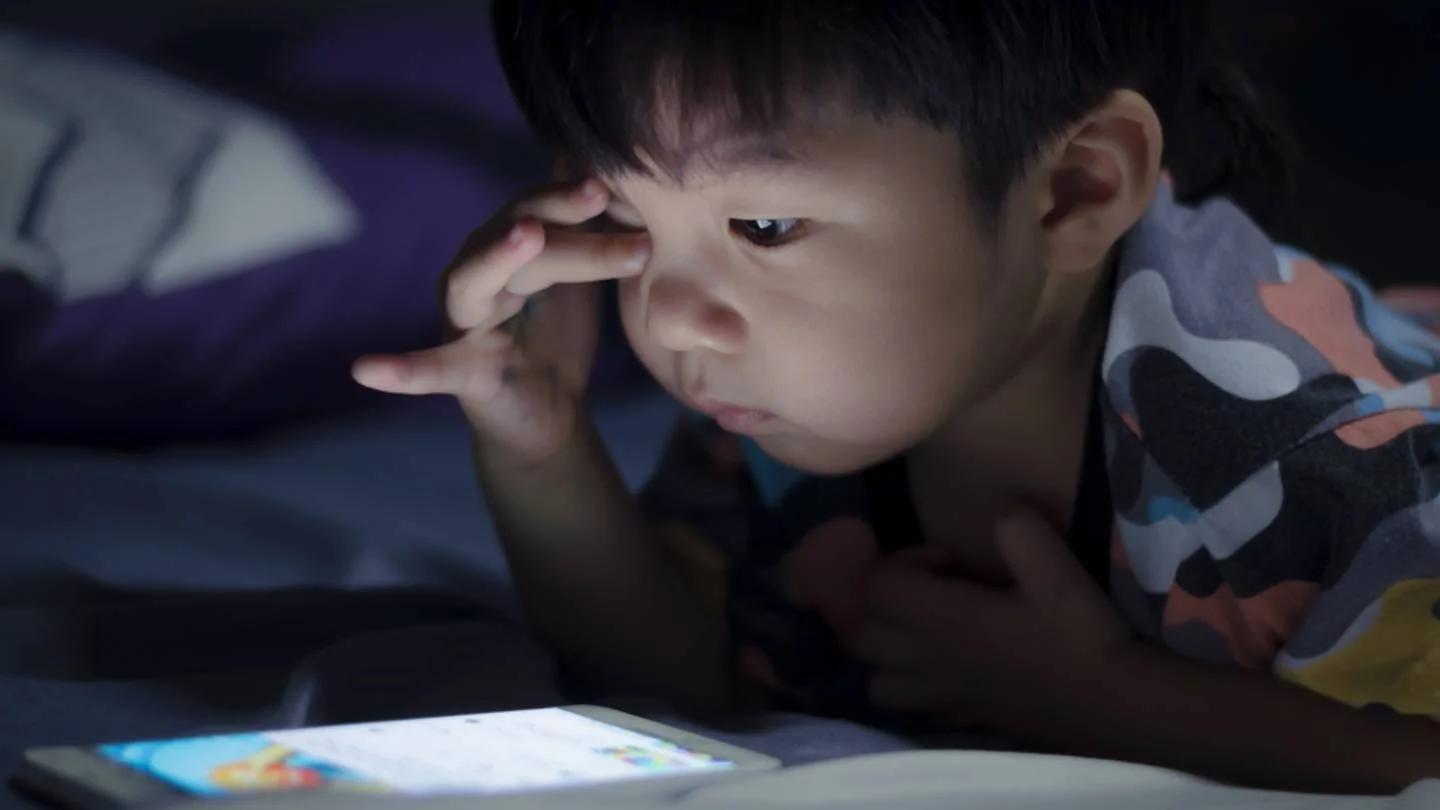
\includegraphics[width=\textwidth]{images/child.png}
        \label{fig:child}
    \end{figure}    
\end{columns}
\end{frame}

% % \textcolor{PGBlack}{\includepdf[pages={1}]{../Article/article.pdf}}


\begin{frame}{Koniec}
    \begin{center}
        {\huge Dziękujemy za uwagę!}
    \end{center}
\end{frame}

\setbeamercovered{transparent}
\begin{frame}[allowframebreaks]{Bibliografia}
    \printbibliography
\end{frame}

\pglastframe

\end{document}